

As demonstrated by the work done for SAVAT and FASE, computing devices generate electromagnetic (EM) emanations when they operate. While previous research has demonstrated that useful information about a system's behavior may be embedded in these emanations (\eg \cite{Rao02a,genkin_2014,CALLAN2014}), it also suggested that such information extraction on devices with highly optimized microarchitecture can be difficult in practice. Nearly all existing techniques for extracting information from EM emanations are used for side channel analysis in cryptography, and are thus focused on extracting information about {\em a specific value used by the program}, such as a cryptographic key.  Furthermore, these techniques operate in an adversarial context; that is, they must overcome program and hardware features (countermeasures) that are specifically designed to mask or obfuscate the impact that the desired data values have on EM emanations.

Profilers have a few advantages over side-channel attackers. First, the profiled system is cooperative, so there are no countermeasures in place, and the profiler may position probes wherever needed to get the best EM signal. Also, program profilers record statistics about when and how often parts of a program execute and are not primarily focused on data values. Sequences of instructions and control flow decisions affect EM emanations more strongly than changes in data values, potentially making profiling information easier to extract than data values.

While the details of how computing devices generate EM emanations are complex, a brief example describing the EM emanations produced by a processor's clock may provide some helpful insight into the connection between EM emanations and program behavior. At each cycle of a processor clock, the processor state is updated, generating a current at the clock's frequency.  Conceptually, the amplitude of this current depends on how much of the processor state changes at each cycle; that is, the current depends on which instructions are active or have been recently executed.  As a program executes, the processor executes different instructions based on control flow decisions, and this variation in instruction execution modulates the amplitude of the processor clock current. EM emanations from the processor can be directly related to the current drawn by the processor. These phenomena together create a direct link between the processor clock EM emanations and program behavior. \zop\ uses this link to determine which code executes and how frequently.

% Alex: the next paragraph is a bit confusing.
If a program executes several times with the same inputs, the waveforms of the EM emanations recorded during program execution may vary significantly between program runs. EM noise from other devices, radio broadcasts, or communication signals can cause these run-to-run variations. However by demodulating the signal at the frequency of the processor clock, one can filter out any noise outside of the narrow band of the RF spectrum around that clock frequency. Furthermore, specially designed EM probes and signal processing can be used to filter out noise with properties distinguishable from our signal of interest (\eg eliminate noise and signals not generated by the processor). In addition to external noise, system activity unrelated to the program and the accumulation of small timing differences caused by the complexity of the system (\eg cache and memory behavior) can also create run-to-run variations between repeated executions with the same inputs. However, these variations are usually smaller than the waveform differences created by execution of different paths through the program. Therefore, by observing a sufficient number of dynamic instances of the same static path, it is possible to later recognize this path by matching it against one of its dynamic instances. For example, if a short path has two dynamic instances, one with a cache miss and one with a cache hit, it is possible to recognize this path as long as there are examples of both possible dynamic instances. We will explain in Section~\ref{sec:profiling} how the ability to recognize short paths can be used to predict complete paths through a program.

\begin{figure}[htb]
  \center
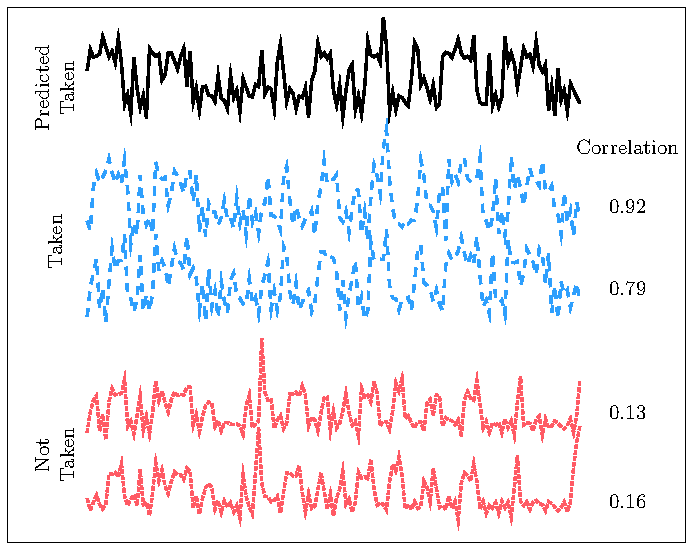
\includegraphics[width=5in]{../issta_profile/profiling/figures/branch_predict}
\caption{Examples of waveforms collected by measuring EM emanations produced by several executions.}
\label{fig:branch_predict}
\end{figure}

Figure~\ref{fig:branch_predict} shows several waveforms recorded during a short fragment of program execution. All of these waveforms start at the same static location in the program, and each follows one of two paths depending on whether the $true$ or the $false$ path of a conditional statement is followed. In particular, the dashed waveforms correspond to execution along the $true$ (conditional branch instruction is ``taken'') path, whereas the two dotted waveforms correspond to execution along the $false$ path (branch instruction is ``not taken''). Assume we use dynamic analysis to determine whether the branch is taken for these cases. It is clear from Figure~\ref{fig:branch_predict} that while there are some differences between these ``training'' waveforms that correspond to the same path, these differences are smaller than those between the $true$ and $false$ paths. To determine which path was taken in the ``unknown'' (solid) waveform without doing any dynamic analysis, we calculate the correlation coefficient between that unknown waveform and each of the candidate recorded waveforms. By observing correlation coefficients, we are able to determine with high confidence that the branch was taken in the unknown execution, as the branch-taken examples correlate much better with it than the branch-not-taken examples.

% reviewer 3: Compare ZOP to a “dumb” approach that just guesses based on likelihood
% \alex{General question: How would our result compare to an approach
%   that uses symbolic analysis for this? Did anybody try that?}
